\documentclass[10pt,conference,compsocconf]{IEEEtran}
\usepackage{booktabs}
\usepackage{tabularx}
\usepackage[english]{babel}
\usepackage[ruled]{algorithm}
\usepackage{algpseudocode}
\usepackage{color}
%\let\labelindent\relax
%\usepackage{enumitem}
\let\proof\relax
\let\endproof\relax 
\usepackage{amsthm}
\usepackage[cmex10]{amsmath}
\usepackage{amsfonts}
\usepackage{multicol}
%\let\subcaption\relax
\usepackage[font=small]{subcaption}
\usepackage{graphicx}
\usepackage[hidelinks,bookmarks=false,pdfpagelabels]{hyperref}
\usepackage[nocompress]{cite}
\usepackage{listings}

% definition environment
\newtheorem{definition}{Definition}
\newtheorem{theorem}{Theorem}
\newtheorem{lemma}{Lemma}
\newtheorem{invariant}{Invariant}

% typewriter font family that support hyphenation
%\newcommand\textvtt[1]{{\normalfont\fontfamily{cmvtt}\selectfont #1}}
\hyphenation{MD-List} 
\hyphenation{skip-list}

\algtext*{EndWhile}
\algtext*{EndFor}
\algtext*{EndIf}
\algtext*{EndFunction}
\newcommand\NIL{\text{NIL}}
\newcommand\TRUE{\text{\textbf{true}}}
\newcommand\FALSE{\text{\textbf{false}}}
\newcommand\BREAK{\text{\textbf{break}}}
\newcommand\CONTINUE{\text{\textbf{continue}}}
\newcommand\AND{\;\text{\textbf{and}}\;}
\newcommand\OR{\;\text{\textbf{or}}\;}
\newcommand\INSERT{\text{\textbf{Insert}}}
\newcommand\DELETE{\text{\textbf{Delete}}}
\newcommand\SUCCEED{\text{\textbf{Succeeded}}}
\newcommand\FAIL{\text{\textbf{Failed}}}
\newcommand\INPROGRESS{\text{\textbf{InProgress}}}
\algrenewcommand\algorithmicindent{1em}

\algblockdefx[StructBlock]{Struct}{EndStruct} [1]{\textbf{struct} #1} [0]{}
\algtext*{EndStruct}
\algblockdefx[EnumBlock]{Enum}{EndEnum} [1]{\textbf{enum} #1} [0]{}
\algtext*{EndEnum}
\algblockdefx[ClassBlock]{Class}{EndClass} [1]{\textbf{class} #1} [0]{}
\algtext*{EndClass}
\algblockdefx[MacroBlock]{Define}{EndDefine} [1]{\textbf{define} #1} [0]{}
\algtext*{EndDefine}
\algblockdefx[InlineBlock]{Inline}{EndInline} [2]{\textbf{inline function} \textsc{#1}(#2)} [0]{}
\algtext*{EndInline}
\algblockdefx[SwitchBlock]{Switch}{EndSwitch} [1]{\textbf{switch} (#1)} [0]{}
\algtext*{EndSwitch}

\begin{document}

\title{Lock-free Transactions without Rollback for Linked Data Structures}

\author{\IEEEauthorblockN{Deli~Zhang\hspace{14pt} Damian~Dechev}
    \IEEEauthorblockA{Department of Computer Science\\
        University of Central Florida\\
        Orlando, FL 32817, USA\\
    de-li.zhang@knights.ucf.edu \hspace{14pt} dechev@eecs.ucf.edu}
}

\maketitle

\begin{abstract}
    Non-blocking data structures allow scalable and thread-safe accesses to shared data. 
    They provide individual operations that appear to execute atomically.
    However, it is often desirable to execute multiple operations atomically in a transactional manner.
    This is nearly impossible without revamping the data structures' intricate underlying design.
    In this work, we present a new methodology for implementing high-performance lock-free transactional linked data structures.
    Our novel technique allows transactions to insert into the data structure logically inactive nodes, which are invisible to operations outside the scope of the transaction.
    We implement a shared transaction descriptor that atomically activates all nodes within a transaction upon committing.
    Comparing to generic approaches, such as software transactional memory (STM) and transactional boosting, our approach leverages the semantic knowledge of the data structure implementation to eliminate the overhead of false conflict and operation roll back.
    In our experimental evaluation using randomly generated transactions, our approach outperforms the state of the art STM approaches by as much as $500\%$ across all scenarios.
\end{abstract}

%\category{D.1.3}{Concurrent Programming}{Algorithms}
%\terms{Algorithms, Performance}
\begin{IEEEkeywords}
    Concurrent Data Structure, Transactional Memory, Lock-free 
\end{IEEEkeywords}

%TODO: define linearizable
%TODO: define CAS
%TODO: define existing node and active node
%TODO: define status of transaction live/committed/aborted transactions

\section{Introduction}
\label{sec:intro}
%TODO: define "state of ADT"/"abstract state of the shared object" 
%TODO: either define "layer of indirection" or avoid using it as a term and replace it with something else
With the growing prevalence of multi-core systems numerous highly concurrent non-blocking data structures have emerged~\cite{linden2013skiplist,ellen2010non,braginsky2012lock,zhang2015lockfree,michael2002high}.
Researchers and advanced users have been using libraries like LibCDS~\footnote{http://libcds.sourceforge.net/}, Tervel~\footnote{http://ucf-cs.github.io/Tervel/} and Intel's TBB~\footnote{https://www.threadingbuildingblocks.org/}, which are packed with efficient concurrent implementations of fundamental data structures.
High level programming languages such as C\#, JAVA and Scala also introduce concurrent libraries, which allow users who are unaware of the pitfalls of concurrent programming to safely take advantage of the performance benefits of increased concurrency.
These libraries provide operations that appear to execute atomically when invoked individually.
However, they fall short when users need to execute a sequence of operations atomically (i.e., compose operations in the manner of a transaction).
For example, given a concurrent map data structure, the following code snippet implementing a simple \texttt{ComputeIfAbsent} pattern~\cite{golan2013concurrent} is error prone.
\begin{lstlisting}[basicstyle=\small,language=JAVA]
    if(!map.containsKey(key)) {
        value = ... // some computation
        map.put(key, value); }
\end{lstlisting}
The intention of this code is to compute a value and store it in the map, if and only if the map does not already contain the given key.
The code snippet fails to achieve this since another thread may have stored a value associated with the same key right after the execution of \texttt{containsKey} and before the invocation of \texttt{put}.
As a result, the thread will overwrite the value inserted by the other thread upon the completion of \texttt{put}.
Programmers may experience unexpected behavior due to the violation of the intended semantics of \texttt{ComputeIfAbsent}.
Many Java programs encounter bugs that are caused by such non-atomic composition of operations~\cite{shacham2011testing}.
Because of such hazards, often users are forced to fall back to locking and even coarse-grained locking, which has a negative impact on performance and annihilates the non-blocking progress guarantees provided by some concurrent containers.

The problem of implementing high-performance transactional data structures~\footnote{Also referred as \emph{atomic composite operations}~\cite{golan2013concurrent}} is important and has recently gained much attention~\cite{golan2013concurrent,bronson2010transactional,herlihy2008transactional,gramoli2013composing,golan2015automatic,hassan2014integrating,koskinen2010coarse}. 
In this paper, we refer to a transaction as sequence of atomic operations on a concurrent data structure~\footnote{This can be seen as a special case of memory transactions where the granularity of operation is on the data structure level instead of memory word level.}.
We consider a concurrent data structure ``transactional'' if it supports executing transactions 1) atomically (i.e., if one operation fails, the entire transaction should abort), and 2) in isolation (i.e., concurrent executions of transactions appears to take effect in some sequential order).
%Supporting transactional operations in concurrent sets~\cite{bronson2011composable} are especially rewarding, because they are the fundamental building blocks of in-memory databases~\cite{}.

General purpose software transactional memory (STM)~\cite{shavit1997software,herlihy2003software} can be used to easily construct transactional data structures from their sequential counterparts: operations executed within an STM transaction are guaranteed to be transactional.
Despite the appeal of straightforward implementation, this approach has not gained practical acceptance due to its significant runtime overhead~\cite{cascaval2008software}.
An STM instruments threads' memory accesses by recording the locations a thread read in a \emph{read set}, and the locations it wrote in a \emph{write set}. 
Conflicts are detected among the \emph{read/write sets} of different threads. 
In the presence of conflicts, only one transaction is allowed to commit while the others are aborted and restarted.
Apart from the overhead of memory instrumentation, excessive transaction aborts in the presence of data structure "hot-spots" (memory locations that are constantly accessed by threads, e.g., the head node of a linked list) limit the overall concurrency~\cite{herlihy2008transactional}.
\begin{figure}[h]
    \centering
    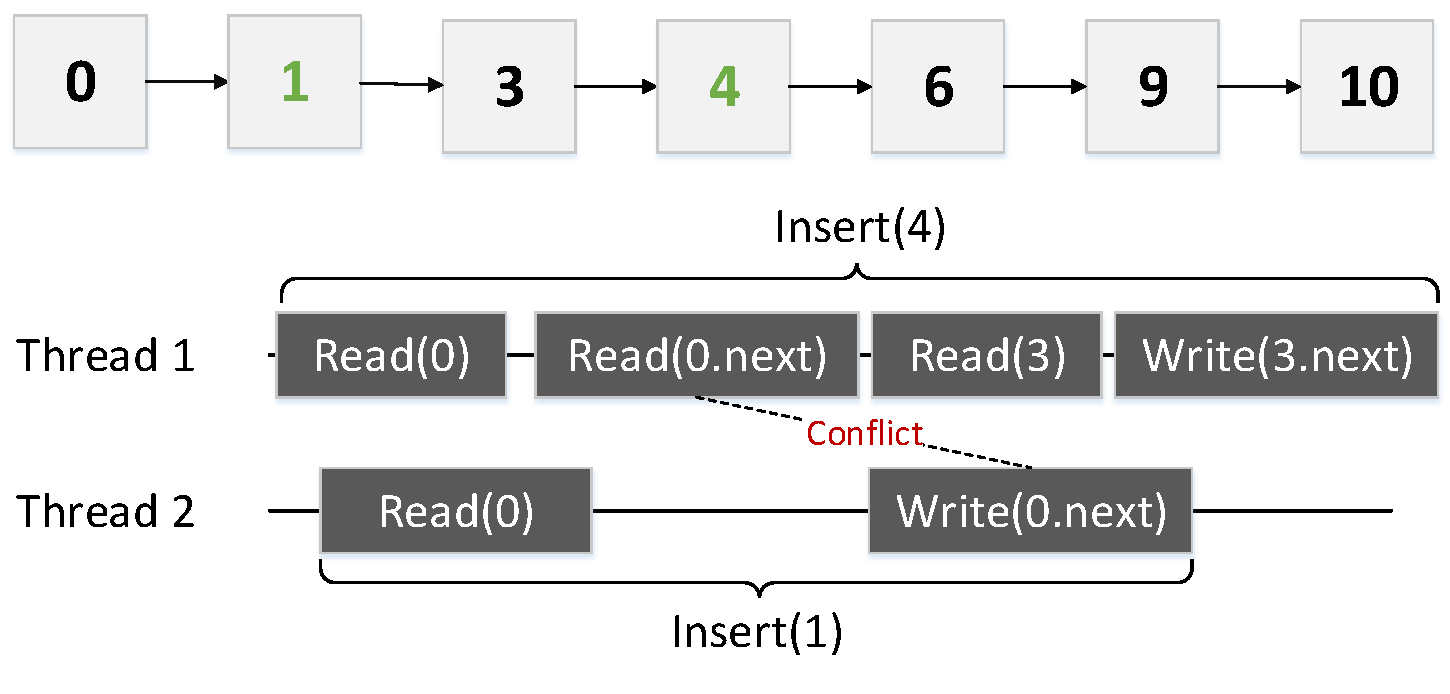
\includegraphics[width=0.8\columnwidth]{figure/stmconflict.pdf}
    \caption{False Conflict in STM}
    \label{fig:stmconflict}
\end{figure}
Figure~\ref{fig:stmconflict} illustrates such an example.
It shows a set implemented as an ordered linked list, where each node has two fields, an integer value and a pointer to the next node.
The initial state of the set is $\{0,3,6,9,10\}$.
Thread 1 and Thread 2 intend to insert 4 and 1, respectively.
Since these two operations commute, it is feasible to execute them concurrently~\cite{clements2015scalable}.
In fact, concurrent linked list implementations employing lock-free~\cite{michael2002high} or fine-grained locking synchronizations~\cite{bayer1977concurrency} allow concurrent execution of the two operations.
Nevertheless, these operations have a read/write conflict and the STM has to abort one of them. 
The inherent disadvantage of STM concurrency control is that low-level memory access conflicts do not necessarily correspond to high-level semantic conflicts.
%Some efforts have be done to alleviate the situation by somehow inferring part of the semantic either through user annotation or.

Transactional boosting~\cite{herlihy2008transactional} is a methodology for transforming linearizable concurrent data structures into transactional data structures.
The basic idea behind boosting is intuitive: if two operations commute they are allowed to proceed without interference (i.e., thread-level synchronization happens within the operations); otherwise they need to be synchronized at the transaction level.
It treats the original data structure as a black box and uses \emph{abstract locking} to ensure that non-commutative method calls do not occur concurrently. 
For each operation in a transaction, the boosted data structure calls the corresponding method of the underlying linearizable data structure after acquiring the abstract lock associated with that call. 
A transaction aborts when it fails to acquire an abstract lock, and it recovers from failure by invoking the inverses of already executed calls. 
This approach eliminates the excessive aborts associated with STM-based transactional data structures, but it still suffers from performance penalties associated with the rolling back of partially executed transactions.
Moreover, in case of non-blocking algorithms, the progress guarantee of the boosted data structure is degraded because of the use of locks for transactional-level synchronization.
%\begin{figure}[h]
    %\centering
    %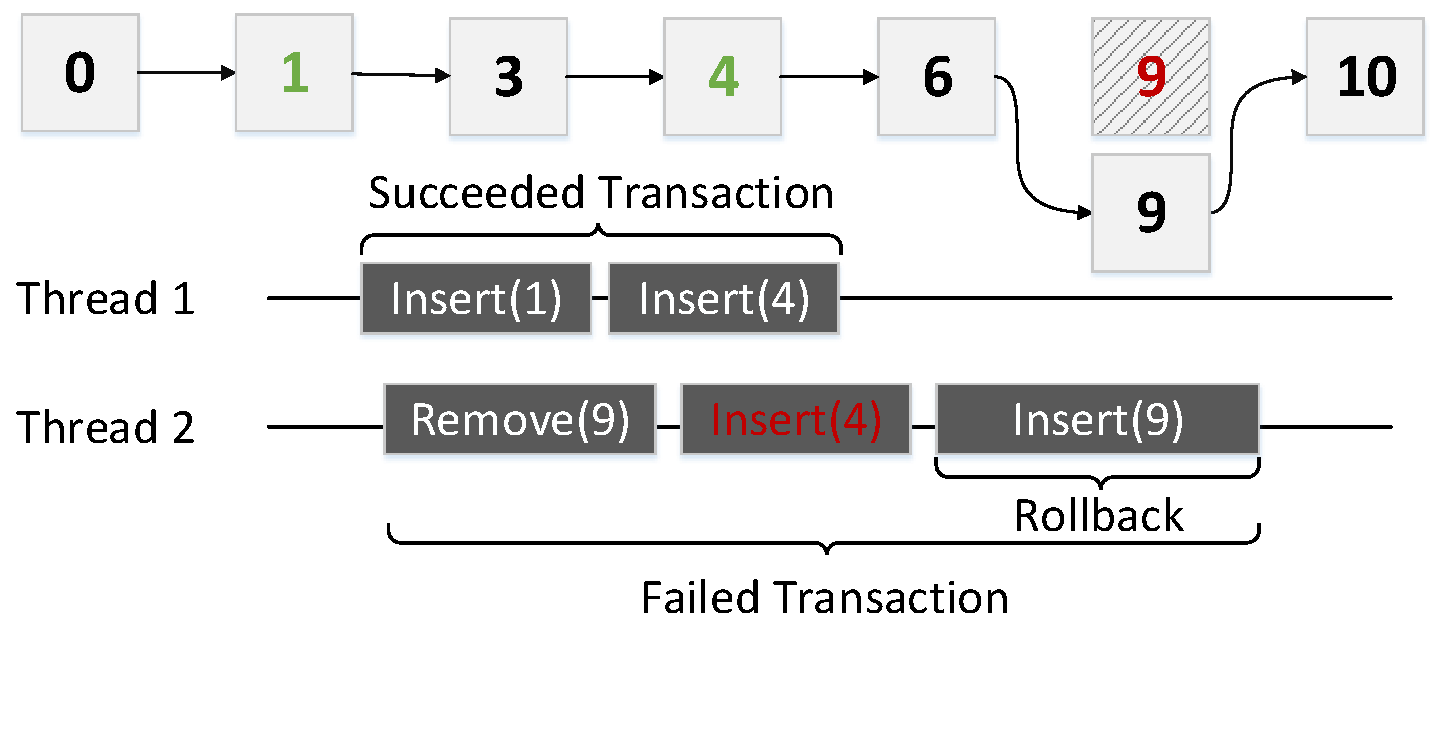
\includegraphics[width=0.9\columnwidth]{figure/boosting.pdf}
    %\caption{Rollbacks in Transactional Boosting}
    %\label{fig:boosting}
%\end{figure}
%In the boosted linked list shown in Figure~\ref{fig:boosting}, the abstract lock is pertaining to each key.  
%thread 1 tries to execute \texttt{Insert(1)} and \texttt{Insert(4)} in a transaction while thread 2 tries to execute \texttt{Remove(9)} and \texttt{Insert(4)} transactionally.
 
In this paper we present a methodology for implementing high-performance lock-free transactional linked data structures without rollback by relying only on the single-word \texttt{ComapreAndSwap} synchronization primitive.
By a linked data structure we mean one that comprises a set of data nodes organized by references. 
Each node has one inbound reference and can have one (e.g., linked list), two (e.g., binary tree), or more (e.g., B-tree and multi-dimensional linked list) outbound references.
Consider the three basic write operations one can perform on a node: insert, delete, and update.
%TODO: think whether the operations indeed act directly, how about those using descriptors?
In existing lock-free implementations, these operations act directly on different fields of a node, and the effects are rendered immediately in the state of the abstract data type (ADT).
We address the two key challenges of supporting transactional operations without rollback: 1) transaction isolation requires that the effects of an operation are invisible to operations outside the transaction's scope before the transaction successfully commits; and 2) delete and update operations require buffering such that their effects can be muted in case of transaction failure.

%TODO: Break this sentence in two: 1st sentence focus on the use of "logical status"; and 2nd sentence: how we implement it
% In 1st sentence, include a "bridge" from the previous paragraph, such as: "To overcome these challenges ..."
At its core, our approach associates a logical status with each node by embedding a reference to a \emph{transaction descriptor} in every node.
A \emph{transaction descriptor} is shared among all nodes within the same transaction, and it stores the operations' context as well as a flag indicating the status of the transaction (e.g., in-progress, succeeded or failed).
A node's logical status denotes how other concurrent operations interpret the node's content.
%and it is determined by the type of operation and the status of the transaction.
Based on the status of the transaction, we categorize nodes into logically active ones and inactive ones.
The logically active nodes are those with a descriptor indicating transaction success, while the logically inactive nodes are those with a descriptor indicating an in-progress or failed transaction.
Logically inactive nodes will be treated by operations outside the transaction scope as ``invisible'', and do not affect the state of the ADT. 
As a result, the state of the ADT is determined by the logically active nodes only.
For example, if a transaction inserted a new node but failed afterwards due to semantic conflicts, the newly inserted node will have a descriptor indicating the transaction failure.
All subsequent operations will proceed as if the node does not exists.

The use of logical status can postpone the effect of an insert operation until the transaction commits.
Delete and update operations in existing data structures cannot exploit this benefit because they do not insert nodes. 
In order to postpone the effect of delete and update operations, we need a layer of indirection, which will enable us to engineer all three write operations in a uniform manner.
We thus design a lock-free node replacement algorithm that allows update or delete operations to insert new nodes that replace exiting nodes in the data structure.
For example, if a transaction needs to delete an existing node, it replaces the old node with a new node, which has the same key as the target node. 
The newly inserted node has a descriptor pertaining to the transaction that executes the delete operation.
If this transaction succeeds, the logical status of the newly inserted node will be interpreted as deleted. 
Otherwise, this implies a failed deletion hence the logical existence of the node.

%TODO: Expand the section on contributions; more assertive language; focus on contributions
%TODO: make sure that you spell it out directly that this is the first lock-free transactional technique that does not use rollback
Our approach has the following algorithmic characteristics:
\begin{itemize}
    \item Lock-free thread-level synchronization provides comparable level of parallelism as the state-of-the-art concurrent data structures;
    \item In-progress and failed transactions do not alter the state of abstract date types;
    \item Serialization is achieved through helping mechanism, thus transactions do not abort upon node access conflict; 
    \item Rolling back executed operations in failed transactions is not necessary as the nodes will remain logically inactive;
\end{itemize}

%TODO: Say that we applied our methodology to implement a linked-list and binary search tree
In our experimental evaluation, we compare transactional linked lists and skip-lists built on RSTM~\cite{marathe2006lowering}, transactional boosting~\cite{herlihy2008transactional}, and our approach on a 64-core NUMA and a 12-core SMP system for transactions with up to 64 operations.
RSTM is the best available object-based non-blocking STM implementation, which provides significant performance advantage over traditional lock-based and data-based STM implementations.
The result shows that on both systems our algorithms achieve more than $500\%$ speedup over RSTM based approaches.
Moreover, on both systems our algorithms outperform transactional boosting approaches by an average of $30\%$ for transactions with more than 4 operations.
%TODO: make a note for a future extended version: compare against basic lock-free linked-list and lock-free binary search tree

The rest of the paper is organized as follows. 
In Section~\ref{sec:related}, we review existing approaches on constructing transactional data structures.
In Section~\ref{sec:algorithm}, we explain our algorithms in details.
We present the transactional linked list in Section~\ref{sec:application}.
We reason about the correctness and progress properties of our algorithms in Section~\ref{sec:correctness}.
The performance evaluation is presented in Section~\ref{sec:experiment}.
We conclude the paper in Section~\ref{sec:conclusion}.
%TODO: in conclusion talk about "the limitation" of supporting linked data structures and the possibility to expand the methodology to others with contiguous memory

\section{Related Work}
\label{sec:related}
%1: lock-free data structures with thread-level synchronization techniques
%2: transaction synchronization
Non-blocking linked data structures have been extensively studied because their distributed memory layout provides data access parallelism and scalability under high levels of contention~\cite{linden2013skiplist,zhang2015lockfree,michael2002high}.
To the best of our knowledge, there is no existing linked data structure that provides native support for transactions.
A transactional execution of data structure operations can be seen as a restricted form of \emph{software transactions}~\cite{harris2010transactional}.
%The scope of the data and the are well defined according to the semantics of the data structure.
%This opens up opportunity for enabling data structure specific optimizations. 
%The users of concurrent data structures have to devise their own concurrency control scheme. 
Straightforward generic constructions can be implemented by executing all shared memory accesses in coarse-grained \emph{atomic sections}, which can employ either optimistic (e.g., STM) or pessimistic (e.g., lock inference) concurrency control.
More sophisticated approaches~\cite{bronson2010transactional,herlihy2008transactional,golan2015automatic} exploit semantic conflict detection for transaction level synchronization to reduce benign conflicts.
%In our work, we combine both fine-grained thread-level synchronization found in existing lock-free data structures and semantic conflict detection to implement transactional linked data structures without the overhead of atomic section synchronizations.

\subsection{Transactional Memory}
Initially proposed as a set of hardware extensions by Herlihy and Moss~\cite{herlihy1993transactional}, transactional memory was intended to facilitate the development of lock-free data structures.
%Even with Intel's recent release of commercial support of best-effort hardware transaction memory (HTM) in their Haswell processors, 
However, due to current HTM's cache-coherency based conflict detection mechanism, transactions are subject to spurious failures during page faults and context switches~\cite{dice2009early}.
This along with excessive aborts under moderate contention~\cite{christina2015resource} make HTM less desirable for implementing transactions in non-blocking data structures.
Thus, considerable amount of work and ingenuity has instead gone into designing lock-free data structures using low-level synchronization primitives such as \texttt{CompareAndSwap}, which empowers researchers to devise algorithm-specific fine-grained concurrency control schemes.

The first software implementation of transactional memory was proposed by Shavit and Touitou~\cite{shavit1997software}, which only supports a static set of data items.
Over the years, improvements have been achieved in terms of functionality~\cite{herlihy2003software}, consistency properties~\cite{guerraoui2008correctness}, progress guarantees~\cite{marathe2006lowering}, and performance~\cite{saha2006mcrt,dice2006transactional}. 
Despite heavy research investment, there is an increasing realization that the read/write conflicts inherently provide insufficient support for concurrency when shared objects are subject to contention~\cite{koskinen2010coarse}.
Meanwhile as design choices have been exhaustively explored~\cite{marathe2004qualitative,marathe2004design}, other limitations faced by STM with regard to usability~\cite{Rossbach2010transactional}, performance~\cite{cascaval2008software}, and expressiveness~\cite{guerraoui2008obstruction} also began to surface.
It has been suggested that STM may not deliver the promised efficiency and simplicity for all scenario, and multitude of approaches should be explored catering to different needs~\cite{attiya2010inherent}.
Unlike STM-based data structures, our approach eliminate false conflict and excessive aborts by adopting semantic conflict detection.

\subsection{Lock Inference}
The STM implementations are typically \emph{optimistic}, which means they execute under the assumption that interferences are unlikely to occur.
They also maintain computationally expensive undo-logs to allow rollback in case a transaction experiences interference.
In light of this shortcoming, pessimistic alternatives based on lock inference has been proposed~\cite{mccloskey2006autolocker}.
These algorithms synthesize enough locks through static analysis to prevent data races in atomic sections.
The choice of locking granularity has an impact on the trade-off between concurrency and overhead.
Some approaches require programmers' annotation~\cite{golan2013concurrent} to specify the granularity, others automatically infer locks at a fixed granularity~\cite{emmi2007lock} or even multiple granularities~\cite{cherem2008inferring}.
Nevertheless, most approaches associate locks with memory locations, which may lead to reduced parallelism due to false conflicts as seen in STM. 
Applying these approaches to real-world programs also faces scalability changes in the presence of large libraries ~\cite{gudka2012lock} because of the high cyclomatic complexity~\footnote{A measure of the number of linearly independent execution paths~\cite{mccabe1976complexity}.} involved in the static analysis process.
Moreover, the use of locks degrades any non-blocking progress guarantee one might expected from using a non-blocking library.
In contrast, our approach guarantees lock-free progress.
%Kempf2014combining combines lock inference and stm.

\subsection{Semantic Conflict Detection}
Considering the imprecise nature of data-based conflict detection, semantic-based approaches have been proposed to identify conflicts at a high-level (e.g., two commutative operations would not raise conflict even though they may access and modify the same data) which enables greater parallelism.
Because semantically independent transactions may have low-level memory access conflicts, some other concurrency control mechanism must be used to protect accesses to the underlying data structure.
This results in a two-layer concurrency control.
Transactional boosting proposed by Herlihy~\cite{herlihy2008transactional} is the first dedicated treatment on building highly concurrent transactional data structures using a semantic layer of abstract locks. 
Transactional boosting is pessimistic in that it acquires locks eagerly before the method calls, but it still requires operation rollback because not all locks are acquired at once.
%PTB, black box design, forfiet data structure specific optimization, need to reverse operation upon failure
Koskinen et al.~\cite{koskinen2010coarse} later generalize this work and introduce a formal framework called coarse-grained transactions.
Hassan et al.~\cite{hassan2014developing} proposed an optimistic version of boosting, which employs a white box design and provides throughput and usability benefits over the original boosting approach.
Other STM variants, such open nested transactions~\cite{ni2007open} support a more relaxed transaction model that leverages some semantic knowledge based on programmers' input.
The relaxation of STM systems and its implication on composability has been studied by Gramoli et al.~\cite{gramoli2013composing}.
The work by Golan-Gueta et al.~\cite{golan2015automatic} apply commutativity specification obtained from programmers' input to inferring locks for abstract data types.
All these approaches require the underlying data structure to be linearizable whereas our approach combines the two layers of synchronization into one.
%TODO: we build transaction sync into thread-level sync to maximize efficiency, enable us to achieve lock-freedom. built-in descriptors
%Our approach, do not track read/write set, highly concurrent, Optimistic lock-free
%we leverage the semantic knowledge of the data structure implementation, 

\section{Methodology}
\label{sec:algorithm}
To ensure atomicity in non-blocking transaction executions, a write operation needs to either buffer or ``hide'' its update until the transaction commits or revert its modifications upon transaction failure.

To achieve a higher degree of efficiency, we follow the former strategy.
Implementing the latter requires extra coordinations between operations in different transaction in order to guarantee isolation.
To effectively ``hide'' the newly inserted nodes before a transaction completes, we embed a logical flag in them, which keeps track of the transaction status. 
This is similar to the \emph{logical deletion} technique, which is used in the lock-free linked list algorithm~\cite{harris2001pragmatic} to ensure list integrity and in the lock-free priority queue algorithms~\cite{linden2013skiplist,zhang2015lockfree} to speedup the \emph{delete-min} process.
Logical deletion encodes a binary logical status in a node's bit-marked next pointer~\cite{harris2001pragmatic}, whereas our approach embeds a multi-value transaction status in the descriptor object shared among nodes.
The key challenge remains to design a deletion and update process that allows logically invisible modification.
We achieve this goal by having these operations insert nodes that are logically inactive instead of removing or modify existing nodes in the data structure.

In this section we explain the data type definition of generic transactional linked data structures. 
We also introduce the core procedures that are shared among different kinds of linked data structures: a) the lock-free node replacement algorithm that converts node deletion and modification into node insertion; and b) the transaction execution procedure that orchestrate concurrent transaction executions.

\begin{algorithm}[h]
    \caption{Node Structures}
    \label{alg:nodestructure}
    \vspace{-0.2in}
    \begin{multicols}{2}
        \begin{algorithmic}[1]
            \Enum{Status}
            \State \textbf{InProgress}
            \State \textbf{Succeeded}
            \State \textbf{Failed}
            \EndEnum
            \Struct{Desc}
            \State \textbf{int} $size$
            \State \textbf{Stauts} $flag$
            \State \textbf{Operation} $ops[\;]$
            \EndStruct
            \Struct{Operation}
            \State \textbf{int} $type,key$
            \State \textbf{void*} $val$
            \EndStruct
            \Struct{Node}
            \State \textbf{int} $key,opid$
            \State \textbf{void*} $val$
            \State \textbf{Node*} $child[N],repl$
            \State \textbf{Desc*} $desc$
            \EndStruct
            \end{algorithmic}
    \end{multicols}
    \vspace{-0.15in}
\end{algorithm}

\begin{algorithm}[h]
    \caption{Pointer Marking}
    \label{alg:pointermarking}
    \begin{algorithmic}[1]
        \State \textbf{const int} $F_{adp} \gets \texttt{0x1}$
        \Define{SetMark}{$(p)$} $(p\;|\;F_{adp})$
        \EndDefine
        \Define{ClearMark}{$(p)$} $(p\;\&\;\sim F_{adp})$
        \EndDefine
        \Define{IsMarked}{$(p)$} $(p\;\&\;F_{adp})$
        \EndDefine
    \end{algorithmic}
\end{algorithm}


\subsection{Data Type Definition}
We define the generic node structure used in the rest of the paper in Algorithm~\ref{alg:nodestructure}. 
A node contains a key-value pair, and an array of child pointers $child[N]$, where $N$ depends on the concrete data type (e.g., 1 for linked lists, 2 for binary trees, etc.)
It also stores a reference to the shared transaction descriptor object $desc$ and an index $opid$ that provides reference to the operation pertaining to this node (i.e., $desc.ops[opid]$ is the operation that inserted this node).
Finally, it has a reference $repl$ to the node it replaces (if it replaces anything).
The descriptor object~\cite{herlihy2012art} \textsc{Desc} is a data structure used in lock-free programming to announce steps that cannot be done by a single atomic instruction.
The functionalities of a transactional descriptor is twofold: 1) it stores all the necessary context for any thread to finish a pending transaction; and 2) it provides the transaction status shared among all nodes participating in the same transaction.
Each \texttt{Operation} structure keeps a key-value pair for the operation and an enumeration of operation type. 
The values of the enumeration should encompass the subset of the concrete data types' application programming interface (API) that supports transactional execution.
We employ the pointer marking technique described by Harris~\cite{harris2001pragmatic} to mark adopted child nodes as well as logically deleted nodes. 
The macros for pointer marking are defined in Algorithm~\ref{alg:pointermarking}.
The $F_{adp}$ flag is co-located with the $child$ pointers.

\begin{figure}[th]
    \centering
    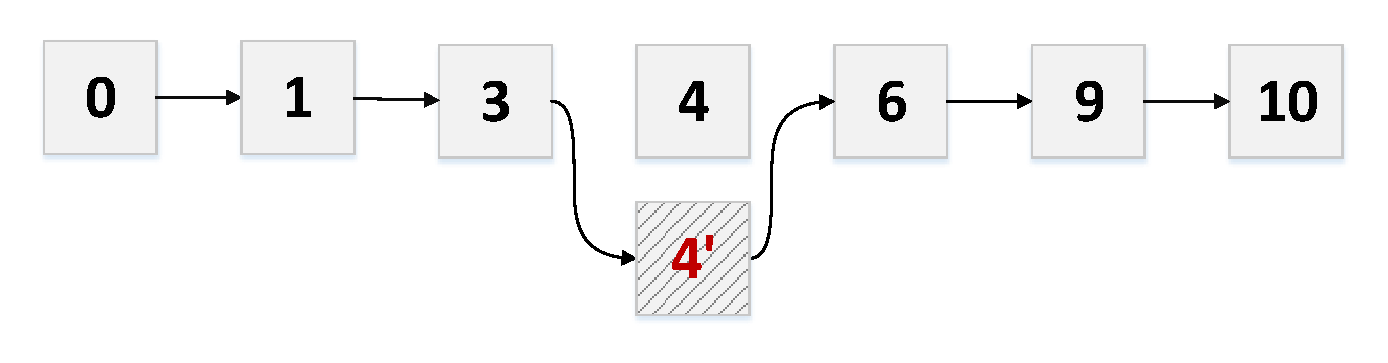
\includegraphics[width=0.8\columnwidth]{figure/deletion.pdf}
    \caption{Node Deletion}
    \label{fig:nodedeletion}
\end{figure}

\begin{algorithm}[th]
    \caption{Node Replacement}
    \label{alg:replace}
    \begin{algorithmic}[1]
        \Function{Replace}{$\textbf{Node*}\;pred,\;\textbf{Node*}\;curr\;\textbf{Node*}\;n,\break\;\textbf{bool}\;replace,\;\textbf{int}\;d_p,\;\textbf{int}\;d_c$}
        \State $n.repl \gets replace = \TRUE \;?\; curr : \NIL$
        \State $n.child[d_c] \gets replace = \TRUE \;?\; \NIL : curr$
        \If {$\text{\textsc{CAS}}(\&pred.child[d_p],\;curr,\;n)$} \label{l:link}
        \State \Call{AdoptChild}{$n$} \label{l:adoptself}
        \State \Return \TRUE
        \Else
        \State \Return \FALSE
        \EndIf
        \EndFunction
        \Statex
        \Function{AdoptChild}{$\textbf{Node*}\;n$}
        %\If {$n = \NIL$}
        %\State \Return
        %\EndIf
        \State \textbf{Node*} $curr \gets n.repl$
        \If {$curr=\NIL \OR \textsc{IsMarked}(curr)$}
        \State \Return
        \EndIf
        \State \textsc{CAS}$(\&curr.repl,\; \NIL,\; \textsc{SetMark}(n)$ \label{l:adoptsetrepl}
        \State \textbf{Node*} $child \gets \NIL$
        \For {$i \in [0, N)$}
        \State $child \gets \textsc{FetchAndOr}(\&curr.child[i],\;F_{adp})$ \label{l:setadp} 
        \State $child \gets \textsc{ClearMark}(child)$
        \State $\text{\textsc{CAS}}(\&n.child[i],\;\NIL,\;child)$ \label{l:adopt}
        \EndFor
        \State $\textsc{CAS}(\&n.repl,\;curr,\;\NIL)$
        \EndFunction
        \end{algorithmic}
\end{algorithm}

\subsection{Lock-free Node Replacement}
\label{sec:noderepl}
All write operations in our approach try to insert new nodes.
If no node with the same key exists, lock-free insertion can be done by simply swinging the next pointer of the predecessor node~\cite{zhang2015lockfree,harris2001pragmatic}. However more often, nodes are inserted to replace an existing node in order to change its logical status.
In Figure~\ref{fig:nodedeletion} we depict the deletion of an existing node (the node labeled with number 4) from a linked-list. 
To perform the operation, in place of the original node we insert a new node (labeled with number 4')
%TODO: explain the helping mechanism of child adoption with graph?
%TODO: make Replace function also insert new node if the node to be replaced is NULL
This requires the child nodes of node being replaced to be transferred to the new node in a lock-free manner.
The \textsc{Replace} function as shown in Algorithm~\ref{alg:replace} inserts a new node $n$ as the $d_p$th child of the predecessor $pred$.
Depending on the boolean flag \textit{replace}, the new node $n$ either replaces $pred$'s original child $curr$ or be positioned between $pred$ and $curr$.
We link $pred.child[d_p]$ to the new node on line\footnote{In the rest of the paper we refer to Line $x$ in Algorithm $y$ as Line x.y}~\algref{alg:replace}{l:link}, and proceed to adopt child nodes from $repl$ in the helper function \textsc{AdoptChild}.
At the beginning of the child adoption process, we store the node pointer $n$ in the $repl$ field of the node that it replaces (line~\algref{alg:replace}{l:adoptsetrepl}).
This back pointer serves as a shortcut for future traversal operations to back track from the replaced node as detailed in Section~\ref{sec:applist}.
Before a child pointer can be copied, we must safeguard it so that it cannot be changed by concurrent insertions while the copy is in progress.
This is done by setting the $F_{adp}$ flag in the child pointers (line~\algref{alg:replace}{l:setadp}).
Once the flag is set either by this thread or by other threads, the function proceeds to copy the pointer to $n$ (line~\algref{alg:replace}{l:adopt}). 
Finally, the descriptor field in $n$ is cleared to designate the operation's completion.

\begin{algorithm}[th]
    \caption{Transaction Execution}
    \label{alg:transaction}
    \begin{algorithmic}[1]
        \Function{ExecuteOps}{$\textbf{Desc*}\;desc,\;\textbf{int}\;opid$}
        \State $ret \gets \TRUE$
        \While {$desc.flag = InProgress$ $\AND ret \AND$ $opid < desc.size$} \label{l:txnwhile}
        \State $\textbf{Operation*} op \gets \&desc.ops[opid]$
        \State $ret \gets \Call{ExecuteOp}{op}$
        \State $opid \gets opid + 1$
        \EndWhile
        \If {$ret = \TRUE$}
        \State $\text{\textsc{CAS}}(\&desc.flag,\;InProgress,\;Succeeded)$ \label{l:txnsuccess}
        \Else
        \State $\text{\textsc{CAS}}(\&desc.flag,\;InProgress,\;Failed)$ \label{l:txnfail}
        \EndIf
        \EndFunction
        \end{algorithmic}
\end{algorithm}


\subsection{Transaction Execution}
\label{sec:txnexec}
%The caveat is that the read operations need to check a node's status to ensure it is in a consistent status or even help the write operation to finish the remaining steps.
In our approach, we treat nodes as the natural units for conflict detection.
%; e.g., insert 3 modifies node 2, but update 3 modifies node 3
Write operations inserting nodes with different keys are allowed to execute concurrently.
Should conflicts among write operations occur, threads help finish the delayed transaction starting from the next operation as indicated by the transaction descriptor in the node in conflict.
The \textsc{ExecuteOps} function in Algorithm~\ref{alg:transaction} execute operations starting from $opid$ in the transaction descriptor $desc$.
The thread initiating the transaction will start from $opid=0$, while other threads may concurrently invoke this method to help unfinished operations with $opid\in[1,desc.size)$.
The method consists of a while loop (line~\algref{alg:transaction}{l:txnwhile}) that executes each operation in order.
The next operation will only be executed if the previous operation completes successfully.
Otherwise, it indicates the precondition required by the previous operation is unsatisfied and the transaction aborts. 
For example, the precondition for a successful deletion operation is that the target key is contained in the data structure.
If this is unsatisfied, the transaction containing such deletion operation will fail.
The concrete \textsc{ExecuteOp} function varies slightly among different data types.
We explain the differences in details in Section~\ref{sec:application}. %TODO: algorithm lists the supported API of a list
Once all operations complete successfully we atomically update the transaction status with a \emph{Succeeded} flag (line~\algref{alg:transaction}{l:txnsuccess}).

\section{Application Examples}
\label{sec:application}
In this section we demonstrate the application of our methodology for implementing transactional linked data structures based on their sequential counterparts. This requires two steps: 1) identifying the conditions that determine if a node is active, and 2) applying the aforementioned lock-free node replacement technique to convert the write operations. The goal of the first step is to construct a sub-routine which helps operations correctly recognize the logical status of a node.
The second step generates uniform write operations that share the same basic node insertion procedure and differ only in the trigger condition for insertion.

%TODO: move node activeness to previous section
\subsection{Linked List}
\label{sec:applist}
We now demonstrate the implementation of a transactional ordered linked list.
%TODO: maybe add 2 sentences as a "teaser" and summary of what was most challenging/interesting about the transformation of the linked-list
Algorithm~\ref{alg:listfind} lists the \texttt{Find} operation as well as four sub-routines that are shared among \texttt{Insert} and \texttt{Delete} operations.
\texttt{Find} determines if a node with a specific key exists.
The node traversal algorithm \texttt{LocatePred}\footnote{We use the notion of reference arguments marked by \textbf{ref}, which surfaces the modification of arguments done by the callee function in the caller function.} locates a node's immediate parent node $pred$ and child node $curr$. 
Similar to the sequential algorithm, termination condition is based on the comparison of the key values (line~\algref{alg:listfind}{l:listpredcheck}).
The child adoption step (line~\algref{alg:listfind}{l:listpredhelp}) is unique to the concurrent algorithm.
It ensures that the child pointer in $curr$ is up to date when read on line~\algref{alg:listfind}{l:listpredchild}

\begin{algorithm}[th]
    \caption{Linked List Find}
    \label{alg:listfind}
    \begin{algorithmic}[1]
        \Function{Find}{$\textbf{int}\;key,\;\textbf{Desc*}\;desc$}
        \State $\textbf{Node*}\;pred \gets \NIL,\;curr \gets head$
        \State \Call{LocatePred}{$pred,\;curr,\;key$}
        \State \Return \Call{ContainKey}{$curr,\;key,\;desc$}
        \EndFunction
        \Statex
        \Function{LocatePred}{$\textbf{ref Node*}\; pred,\;\hfill$ $\textbf{ref Node*}\; curr,\;\textbf{int}\;key$}
        \While {$curr \neq \NIL \AND curr.key < key$} \label{l:listpredcheck}
        \State $pred \gets curr$
        \State \Call{AdoptChild}{$curr$} \label{l:listpredhelp}
        \State $curr \gets \textsc{ClearMark}(curr.child[0])$ \label{l:listpredchild}
        \EndWhile
        \EndFunction
        \Statex
    \Function{ContainKey}{$\textbf{Node*}\; n,\; \textbf{int}\; key,\;\textbf{Desc*}\;desc$}
    \State \Return $\Call{IsExist}{n,key} \AND \Call{IsActive}{n,desc}$ \label{l:listcontain}
        \EndFunction
        \Statex
        \Function{IsExist}{$\textbf{Node*}\; n,\; \textbf{int}\; key$}
        \State \Return $n \neq \NIL \AND n.key = key$ \label{l:listfindexist}
        \EndFunction
        \Statex
        \Function{IsActive}{$\textbf{Node*}\;n,\; \textbf{Desc*}\; desc$}
        \If{$n.desc.status = \INPROGRESS$} \label{l:listactiveinprogress}
        \If{$n.desc = desc$} \label{l:listactivedesc}
        \State \Return $n.desc.ops[n.opid].type = \INSERT$
        \Else
        \State \Call{ExecuteOps}{$n.desc,\;n.opid+1$} \label{l:listactivehelp}
        \EndIf
        \EndIf
        \State $\textbf{Status}\; status \gets n.desc.status$ \label{l:listfindreadstatus}
        \State $\textbf{int}\; type \gets n.desc.ops[n.opid].type$
        \State \Return $(type = \INSERT \AND status = \SUCCEED) \hfill\break \OR (type = \DELETE \AND status = \FAIL)$ \label{l:listactivecond}
        \EndFunction
    \end{algorithmic}
\end{algorithm}

Upon the completion of node traversal, we determine whether the list actually contains target key by two criteria on line~\algref{alg:listfind}{l:listcontain}: 1) the node is found to exist (i.e., it is reachable from the head); and 2) the node is active.
The first condition follows the sequential algorithm and is checked in the \texttt{IsExist} function.
The second condition is checked in the \texttt{IsActive} function.
We consider a node active if it is inserted by an \texttt{Insert} operation and the whole transaction commits successfully, or if it is inserted by a \texttt{Delete} operation and the transaction fails (line~\algref{alg:listfind}{l:listactivecond}).
Moreover, for in-progress transactions (line~\algref{alg:listfind}{l:listactiveinprogress}) we also need to recognize nodes inserted by the \texttt{Insert} operations in the same transaction as active. %TODO: correctness citation
This is done by testing the equality between the current transaction's descriptor and the descriptor of the transaction that inserted the node (line~\algref{alg:listfind}{l:listactivedesc}).
For all other in progress transactions, we invoke the helper method (line~\algref{alg:listfind}{l:listactivehelp}) and obtain the node's activeness after the transaction completes. %TODO: the help method should set status flag if opid is larger than the op size

\begin{algorithm}[t]
    \caption{Linked List Insert}
    \label{alg:listinsert}
    \begin{algorithmic}[1]
        \Function{Insert}{$\textbf{int}\;key,\;\textbf{Desc*}\;desc,\;\textbf{int}\;opid$}
        \State $\textbf{Node*}\; n \gets \text{\textbf{new Node}}$
        \State $n.key \gets key,\;n.val \gets val$
        \State $n.desc \gets desc,\;n.opid \gets opid$
        \State $\textbf{Node*}\; pred \gets \NIL,\;curr \gets head$
        \While{\TRUE} \label{l:listinsertwhile}
        \State \Call{LocatePred}{$pred,\;curr,\;key$}
        \If{\Call{ContainKey}{$curr,\;key,\;desc$}} \label{l:listinsertcontain}
        \State \Return $curr.desc = desc$ \label{l:listinsertdesc}
        \EndIf
        \State $\textbf{bool}\; replace \gets \Call{IsExist}{curr,\;key}$ \label{l:listinsertexist}
        \If {\Call{Replace}{$pred,\;curr,\;n,\;replace,\;0,\;0$}} \label{l:listinsertreplace}
        \State \Return \TRUE \label{l:listinsertreturn}
        \Else
        \State $curr \gets \textsc{IsMakred}(pred.child[0]) \;?\; \hfill \break  \textsc{ClearMark}(pred.repl) : pred$ \label{l:listinsertpred}
        \State $pred \gets \NIL$ 
        \EndIf
        \EndWhile
        \EndFunction
    \end{algorithmic}
\end{algorithm}


\begin{algorithm}[t]
    \caption{Linked List Delete}
    \label{alg:listdelete}
    \begin{algorithmic}[1]
        \Function{Delete}{$\textbf{int}\;key,\;\textbf{Desc*}\;desc,\;\textbf{int}\;opid$}
        \State $\textbf{Node*}\; n \gets \text{\textbf{new Node}}$
        \State $n.key \gets key,\;n.val \gets val$
        \State $n.desc \gets desc,\;n.opid \gets opid$
        \State $\textbf{Node*}\; pred \gets \NIL,\;curr \gets head$
        \While{\TRUE}
        \State \Call{LocatePred}{$pred,\;curr,\;key$}
        \If{$!\Call{IsExist}{curr,\;key}$} \label{l:listdeleteexist}
        \State \Return \FALSE
        \EndIf
        \If{!\Call{IsActive}{$curr,\;desc$}} \label{l:listdeleteactive}
        \State \Return $curr.desc = desc$
        \EndIf
        \If {\Call{Replace}{$pred,\;curr,\;n,\;\TRUE,\;0,\;0$}} \label{l:listdeletereplace}
        \State \Return \TRUE
        \Else
        \State $curr \gets \textsc{IsMakred}(pred.child[0]) \;?\;\hfill \break \textsc{ClearMark}(pred.repl) : pred$ 
        \State $pred \gets \NIL$ 
        \EndIf
        \EndWhile
        \EndFunction
    \end{algorithmic}
\end{algorithm}

Algorithm~\ref{alg:listinsert} lists the \texttt{Insert} function.
After allocating a new node and set its field values, the function enters a CAS-based while loop (line~\algref{alg:listinsert}{l:listinsertwhile}).
The position to insert the new node is given by \texttt{LocatePred}.
Note that on line~\algref{alg:listinsert}{l:listinsertcontain} we check if the list already contains the target key.
If this is the case, we skip the insertion and return result code based on the equality of the transaction descriptors (line~\algref{alg:listinsert}{l:listinsertdesc}).
Due to the use of helping mechanism, the same \texttt{Insert} operation may be executed multiple times by different threads.
This condition check allows us to identify node inserted by other threads that executes the same transaction and thus ensures consistent result code is return for all execution paths.
This is important as all helping threads will try to set the transaction phase flag at the end of the execution; conflicts attempts on setting the transaction phase flag is possible if multiple execution of the same operation do not reach consensus on the result code.
On line~\algref{alg:listinsert}{l:listinsertreplace}, \texttt{Replace} is called to place the new node in the list.
If a node with same key exist but is inactive (line~\algref{alg:listinsert}{l:listinsertexist}), the existing node $curr$ will be replaced by the new node.
Should the CAS operation in \texttt{Replace} fail due to contention, we reset the traverse variable $pred$ and $curr$ and start the loop over again.
The traverse restart point depends on whether $pred$ node has been replaced by some other nodes, which can be inferred from the marked child pointer (line~\algref{alg:listinsert}{l:listinsertpred}).
When $pred$'s child node is marked, $pred$ is no longer reachable from the head.
We restart the traversal from the node that replaces $pred$, whose reference was stored in the $pred$'s $repl$ field during the child adoption process (line~\algref{alg:replace}{l:adoptsetrepl}).
Otherwise, we simply start from $pred$.

The \texttt{Delete} operation listed in Algorithm~\ref{alg:listdelete} shares the same structure as the \texttt{Insert} operation.
The difference is that it inserts the new node when the list contains the target key (line~\algref{alg:listdelete}{l:listdeleteexist} and~\algref{alg:listdelete}{l:listdeleteactive}), and the newly inserted node always replaces an existing active node (the \textit{replace} flag on line~\algref{alg:listdelete}{l:listdeletereplace} is set to true).

\section{Correctness}
\label{sec:correctness}
Using the above linked list as an example, we briefly reason about the safety and progress properties of the transactional data structures constructed using our methodology. 
We start by showing the \texttt{Find}, \texttt{Insert}, and \texttt{Delete} operations are \emph{linearizable}~\cite{herlihy2012art}.
Since a linearizable operation appears to take effect instantaneously at some point between its method invocation and method return, it can be treated as an atomic operation in the context of transaction execution.
We then sketch a proof that the transactional executions of these atomic operations satisfy \emph{opacity}~\cite{guerraoui2008correctness}.
Finally, we show that our algorithm provides lock-free progress. 

\subsection{Linearizability}
Let us consider the case where the maximum number of operations in a transaction is limited to one.
The transactional linked list introduced in Section~\ref{sec:applist} degenerates to a concurrent linked list.
We show that it is a linearizable linked list implementation that complies with the \emph{set} semantics by identifying \emph{linearization points} for each operation.
%The concurrent operation can be viewed as it occurred atomically at its linearization point in the execution history.
We denote the set of keys that are contained by all nodes in the linked list as $U$, and the set of keys that are contained by the inactive nodes as $V$.
The abstract state of the set is then $S \equiv U \setminus V$.
Additionally, we use the notion of decision points and state-read points to facilitate our reasoning. 
The decision point of an operation is define as the atomic statement that finitely decides the result of an operation, i.e. independent of the result of any subsequent instruction after that point.
A state-read point is define as the atomic statement where the state of the dictionary, which determines the outcome of the decision point, is read.

\begin{theorem}
    A $\textsc{Find}(k)$ operation takes effect atomically at one statement.
\end{theorem}
\begin{proof}
    A find operation returns true if $k \in S$, or false otherwise.  
    The decision point for the first case is on line~\algref{alg:listfind}{l:listactivecond} when the list already contains an active node with the same key.
    The decision points for the latter case is on line~\algref{alg:listfind}{l:listfindexist} when it cannot find the node with the target key, and on line~\algref{alg:listfind}{l:listactivecond} when the target node is logically inactive (i.e., already deleted).
    The state-read point and hence the linearization point for both cases is on line~\algref{alg:listfind}{l:listpredchild}, where $curr$ is read.
\end{proof}

\begin{theorem}
    An $\textsc{Insert}(k)$ operation takes effect atomically at one statement.
\end{theorem}
\begin{proof}
    An \textsc{Insert} operation returns true on line~\algref{alg:listinsert}{l:listinsertreturn}; it must have succeeded in either a) adding a new node or b) replacing an existing inactive node.
    The decision point for both cases to take effect is when the CAS operation on line~\algref{alg:replace}{l:link} succeeds.
    The remaining atomic primitives in the child adoption process will be executed at least once (line~\algref{alg:replace}{l:adoptself}) and successfully complete through the use of helping mechanism (line~\algref{alg:listfind}{l:listpredhelp}).
    The abstract state of the set is correctly changed because $U'=U\cup \{ k \}$ (for case a), and $V'=V \setminus \{ k \}$ (for case b).
    The linearization point for a $\textsc{Insert}(k)$ operation to fail is the same if the \textsc{Find} operation succeeds.
\end{proof}

\begin{theorem}
    A $\textsc{Delete}(k)$ operation takes effect atomically at one statement.
\end{theorem}
\begin{proof}
    If $k \in S$, a successful $\textsc{Delete}(k)$ operation changes the abstract state as follows: $V' = V \cup \{k\} \implies S' = S \setminus \{ k\}$
    The decision point as well the linearization point for it to take effect is when the CAS operation on line~\algref{alg:replace}{l:link} succeeds.
    The linearization point for a $\textsc{Delete}(k)$ operation to fail is the same if the \textsc{Find} operation fails.
\end{proof}

\subsection{Opacity}
Our algorithm satisfies opacity~\cite{guerraoui2008correctness}, which is a stronger STM correctness condition than traditional serializability~\cite{papadimitriou1979serializability}.
Intuitively, opacity requires that 1) all operations performed by every committed transaction appear as if they happened at some single, indivisible point during the transaction lifetime, 2) no operation performed by any aborted transaction is visible to other transactions and 3) every transaction (including live transactions) always observes a consistent state of the shared object.
For brevity, we informally reason about how our algorithm meets these requirements.

\begin{lemma} \label{lmm:inactive}
    Nodes inserted by operations in a transaction stay inactive until the transaction commits.
\end{lemma}
\begin{proof}
    Nodes are active iff the transaction status flag is set to \emph{Succeeded}, which is done using CAS on line~\algref{alg:transaction}{l:txnsuccess}.
\end{proof}

\begin{lemma} \label{lmm:inactive1}
    Nodes inserted by operations in a aborted transaction stay inactive.
\end{lemma}
\begin{proof}
    The \emph{Failed} transactions status flag is set using CAS on line~\algref{alg:transaction}{l:txnfail}.
\end{proof}

\begin{lemma}
    Pairwise concurrent transactions have a conflict if and only if they contain operations that access the same key.
\end{lemma}
\begin{proof}
    Since all operations are linearizable, 
\end{proof}

\begin{lemma}
    All transactions including live transactions observe a consistent abstract state of the data structure.
\end{lemma}
\begin{proof}
\end{proof}

\begin{theorem}
    The transactional execution of the linked list operations is opaque.
\end{theorem}
\begin{proof}
Follow Lemma~\ref{lmm:inactive}, opacity requirement 1 is met. 
Follow Lemma~\ref{lmm:inactive1}, opacity requirement 2 is met. 
Follow Lemma~\ref{}, opacity requirement 3 is met. 
\end{proof}

\section{Performance Results}
\label{sec:experiment}
We compare the overhead and scalability of our lock-free transactional list and skiplist against the implementations based on transaction boosting and STMs found in Rochester Software Transactional Memory package\footnote{http://cs.rochester.edu/research/synchronization/rstm/}.
RSTM is the best available comprehensive suite of prevailing STM implementations.
Most of the algorithms distributed with RSTM support building transactional data structures with a few exception such as single lock algorithms and in-place write algorithms. 
Due to their lack of support for explicit self-abort, transactions with failed operations cannot be revoked leading to potentially erroneous behavior.  
In our test, TML~\cite{dalessandro2010norec} and its extension NOrec~\cite{dalessandro2010norec} were the among the fastest on our platform.
They have extreme low overhead and good scalability due to elimination of owner ship records.
We choose NOrec as the representative implementation because its value-based validation allows for more concurrency for readers with no actual conflict.

For transaction boosting, we implemented the lookup of abstract lock using Intel TBB's concurrent hash map.
Although the original transaction boosting was designed to be used in tandem with STMs for replaying undo logs, it is not necessary in our test case as the data structures were tested in isolation.
To reduce the runtime overhead, we scrap the STM environment and implemented a lightweight per-thread undo log for the boosted data structures.
We employ a micro-benchmark to evaluate performance in three types of workloads: write dominated, read dominated, and mixed.
This canonical evaluation method~\cite{dalessandro2010norec,harris2001pragmatic} consists of a tight loop that randomly chooses to perform a fixed size transaction with a mixture of \textsc{Insert}, \textsc{Delete} and \textsc{Find} operations according to the workload type.
We also vary the transaction size (i.e., the number of operations in a transaction) from 1 to 16 to measure the performance impact of rollbacks.
The tests are conducted on a 64-core NUMA system (4 AMD opteron 6272 CPUs with 16 cores per chip @2.1 GHz). 
Both the micro-benchmark and the data structure implementations are compiled with GCC 4.7 with C++11 features and \texttt{O3} optimizations.

\begin{figure*}[t]
    \begin{subfigure}{0.325\textwidth}
        \centering
        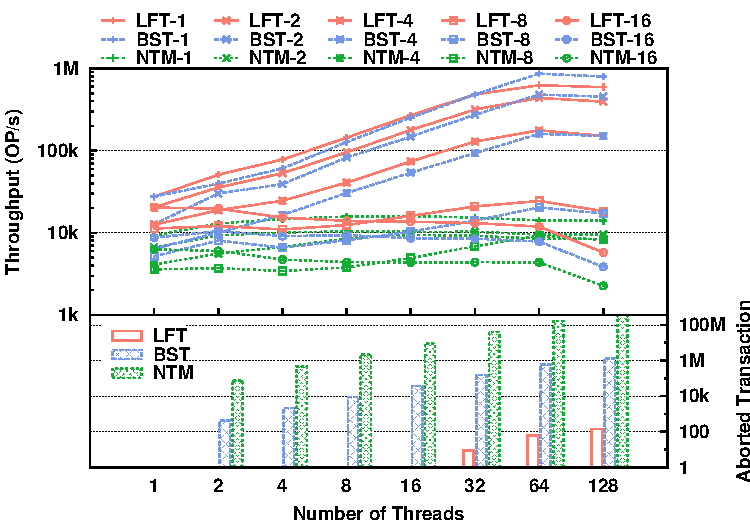
\includegraphics[width=1\columnwidth]{./data/amd50ins10kfilled.pdf}
        \caption{50\% \textsc{Insert}, 50\% \textsc{Delete}, 0\% \textsc{Find}}
        \label{fig:txnlist50}
    \end{subfigure}
    \hfill
    \begin{subfigure}{0.325\textwidth}
        \centering
        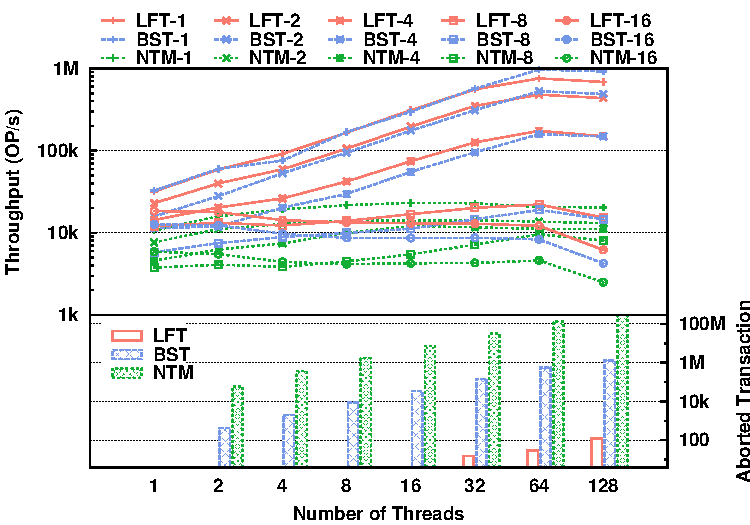
\includegraphics[width=1\columnwidth]{./data/amd33ins10kfilled.pdf}
        \caption{33\% \textsc{Insert}, 33\% \textsc{Delete}, 34\% \textsc{Find}}
        \label{fig:txnlist33}
    \end{subfigure}
    \hfill
    \begin{subfigure}{0.325\textwidth}
        \centering
        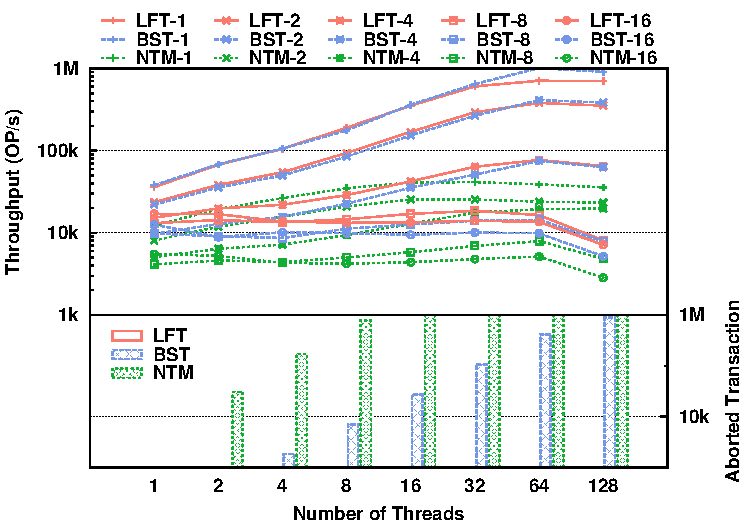
\includegraphics[width=1\columnwidth]{./data/amd15ins10kfilled.pdf}
        \vspace{-0.17in}
        \caption{15\% \textsc{Insert}, 5\% \textsc{Delete}, 80\% \textsc{Find}}
        \label{fig:txnlist15}
    \end{subfigure}
    \caption{Throughput and Superfluous Abort Counts for Transaction Lists (10K Key Range)}
    \label{fig:txnlist}
    \vspace{-0.2in}
\end{figure*}


\subsection{Transactional List}
\label{sec:txnlistexp}
We show the throughput and the number of superfluous aborts in Figure~\ref{fig:txnlist} for all three types of lists.
The throughput is measured in terms of number of completed operations per second, which is the product of the number of committed transactions and transaction size.
The number of superfluous aborts takes into account the number of aborted transactions except self-aborted ones.
This is an indicator for the effectiveness of the conflict management scheme.
Each thread performs 1 hundred thousand transactions and the key range is set up to 10 thousand.
Our lock-free transactional list is denoted by LFT, the boosted list by BST, and the NOrec STM list by NTM. 
The underlying list implementations for both LFT and BST were based on Harris' lock-free design~\cite{harris2001pragmatic}.
The linked list for NTM is taken directly from the benchmark implementation in RSTM suite.
For each list legend annotation, we append a numeric postfix to denote the transaction size (e.g., BST-4 means the boosted list tested with 4 operations in one transaction). 

In Figure~\ref{fig:txnlist50}, threads perform solely write operations.
The upper half of the graph shows the throughput with both $y$- and $x$-axises in logarithm scale.
Starting with transaction of size 1, the throughput curve of BST-1 and LFT-1 essentially expose the overhead difference between the two transaction synchronization schemes.
Because each transaction contains only one operation, the code paths for transaction rollback in BST and transaction helping in LFT will not be taken.
For each node operation, BST-1 needs to acquire and release a mutex lock, while LFT-1 needs to allocate a transaction descriptor.
For executions within one CPU chip (no more than 16 threads), LFT-1 maintain a moderate performance advantage to BST-1, averaging more than 15\% speedup.
As the execution spawns across multiple chips, LFT-1's performance is setback by the use of descriptor, which incurs more remote memory accesses.
This trend can be observed for all scenarios with different transaction sizes.
Another noticeable trend is that LFT lists gain better performance as the transaction sizes grows.
For example, on 64 threads the throughput of LFT-2 slightly falls short behind that of BST-2, then the performance of LFT-4 is on par with BST-4, and finally LFT-8 and LFT-16 outperforms their BST counterpart by as much as 50\%.
Two factors contribute to the great scalability of LFT lists in handling large transactions: 1) its helping mechanism manages conflict and greatly reduces superfluous aborts whereas in BST such aborts cause a significant amount of rollbacks; 2) the number of allocated transaction descriptors decreases as the transaction size grows where as in BST the number of required lock acquisitions stays the same.

Generally, we observe that for small transaction sizes (no more than 4 operations), BST and LFT lists explore fine-grained parallelism and exhibit similar scalability trends.
The throughput increases linearly until 16 threads, and continues to increase at a slower pace until 64 threads.
Because executions beyond 16 threads span across multiple chips, the performance growth is slightly reduced due to the cost of remote memory accesses.
The executions are no longer fully concurrent beyond 64 threads, thus the overall throughput is capped and may even reduce due to context switching overhead.
LFT lists obtain an average of 25\% speedup over BST lists.
For large transactions, the throughputs of both LFT and BST list do not scale well.
This could be attributed to the semantic and the randomness of the benchmark.
As the transaction size grows, the probability of a randomly generated sequence of operations will all succeed is inherently smaller.
Most of the transactions were self-aborted due to some failed attempts to located the target element.
LFT lists outperforms BST lists by an average of 40\% in these scenarios.
On the other hand, the throughput of all NTM lists stagnates as the number of threads increases.
Since NTM uses a single writer lock, concurrency is precluded for this write-dominated test case.
On 64 threads, both BST and LFT lists were able to achieve as much as 10 times better performance than NTM lists.

On the bottom half of Figure~\ref{fig:txnlist50}, we illustrate the histogram of superfluous aborts across all transaction sizes and cluster them by thread counts.
The $y$-axis is in logarithmic scale.
For BST lists and NTM lists the number of superfluous aborts grows linearly with the increase of threads.
BST lists have about 100 times less aborts than NTM lists, which matches our intuition that semantic conflict detection can remarkably reduce the number of false conflicts.
Also as expected no approach incurs superfluous aborts in single thread scenario.
Remarkably, LFT lists did not introduce superfluous aborts until 32 threads, and the number of aborts is 4 orders of magnitude smaller than that of BST lists. 
The helping scheme of LFT were able to resolve majority of the conflict in a cooperative manner, and aborts only when cyclic dependencies exist among transactions.

We show the results from mixed and read-dominated workloads in Figure~\ref{fig:txnlist33} and~\ref{fig:txnlist15}. 
The throughputs follows the same pattern as in Figure~\ref{fig:txnlist50} with LFT lists' performance advantage slightly diminishes in read-dominated workload.
This is because the \textsc{Find} operations in LFT lists also update descriptors in nodes, which requires extra cycle compared with read-only BST \textsc{Find} operations.
Nevertheless, LFT lists still maintain an average of 20\% speedup over BST lists in these scenarios and achieves as much as 40\% throughput gain for large transactions.  
Because of allowing reader concurrency, NTM lists also exhibit some degree of scalability in read-dominated scenarios.

\begin{figure*}[t]
    \begin{subfigure}{0.325\textwidth}
        \centering
        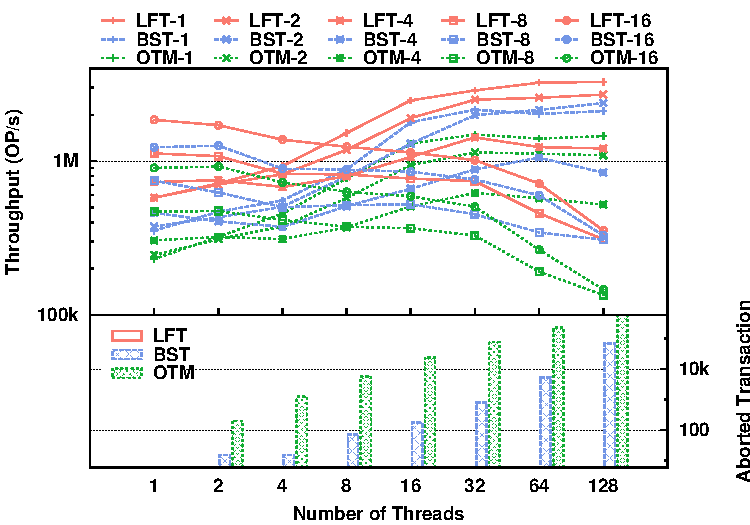
\includegraphics[width=1\columnwidth]{./data/amdskip50ins10kfilled.pdf}
        \caption{50\% \textsc{Insert}, 50\% \textsc{Delete}, 0\% \textsc{Find}}
        \label{fig:txnskip50}
    \end{subfigure}
    \hfill
    \begin{subfigure}{0.325\textwidth}
        \centering
        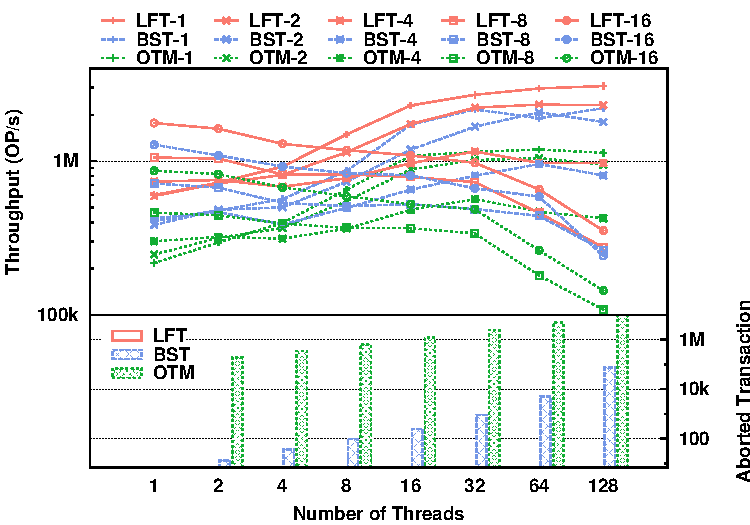
\includegraphics[width=1\columnwidth]{./data/amdskip33ins10kfilled.pdf}
        \caption{33\% \textsc{Insert}, 33\% \textsc{Delete}, 34\% \textsc{Find}}
        \label{fig:txnskip33}
    \end{subfigure}
    \hfill
    \begin{subfigure}{0.325\textwidth}
        \centering
        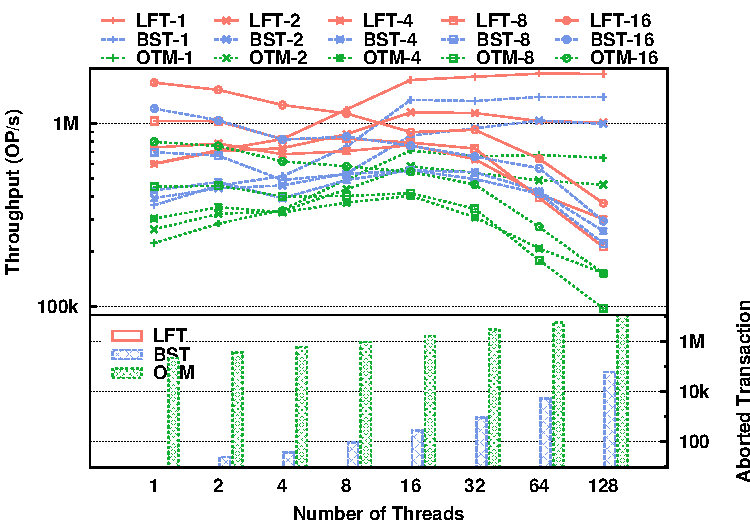
\includegraphics[width=1\columnwidth]{./data/amdskip15ins10kfilled.pdf}
        \vspace{-0.17in}
        \caption{15\% \textsc{Insert}, 5\% \textsc{Delete}, 80\% \textsc{Find}}
        \label{fig:txnskip15}
    \end{subfigure}
    \caption{Throughput and Superfluous Abort Counts for Transaction Skiplists (1M Key Range)}
    \label{fig:txnskip}
    \vspace{-0.2in}
\end{figure*}

\subsection{Transactional Skiplist}
\label{sec:txnskiplistexp}
In Figure~\ref{fig:txnskip}, we show the throughput and the number of superfluous aborts for three types of transactional skiplists.
All of them were based on Fraser's open source lock-free skiplist~\cite{fraser2004practical}. 
The naming convention for BST and LFT skiplists remain the same as in Figure~\ref{fig:txnlist}.
We denote the STM based skiplist as OTM because it uses Fraser's object-based STM.
Compared with word-based STMs, an object-based STM groups memory into blocks thus reduces metadata overhead.
Since skiplists have logarithmic search time, we were able to stress the algorithms with heavier workloads: each threads now performs 1 million transactions and the key range is also boosted to 1 million.

Overall, with a peak throughput of more than 3 million (OP/s), transaction execution on skiplists is considerable more efficient than on linked lists.
Also both OTM and BST skiplists generates 2 orders or magnitude less superfluous aborts than their list counterparts.
Because skiplist algorithms traverse exponentially less nodes than list algorithms, a single operation could finish much sooner, which greatly reduces the probability of memory access conflicts in STM and lock acquisition time out in transaction boosting.
Another noteworthy difference is that the divergent scalability trends of large and small transactions. 
As we can see in in Figure~\ref{fig:txnskip50}, large transaction such as LFT-8 and LFT-16 achieves maximum throughputs on a single thread, then their throughputs steadily fall as the number of thread increases.
On the contrary, the throughputs of small transactions such as LFT-2 and LFT-4 start low, but gain momentum as more threads are added.
Large transactions have lower synchronization overhead but are vulnerable to conflict.
As the number of thread increases, a failed large transaction could easily forfeit a considerable amount of operations.
On the flip side, small transactions incurs greater synchronization overhead, but are less likely to encounter conflicts when more threads contend with each other.
%Transaction lists also exhibits signs of such divergence in Figure~\ref{fig:txnlist} but it is not as significant.

Despite the differences, we still observe performance results generally similar to that of transaction lists.
LFT and BST skiplists outperforms OTM skiplists by as much as 3 times across all scenarios, while LFT skiplists maintain an average of 60\% speedup over BST for large transactions.
For example, in Figure~\ref{fig:txnskip50} on 32 threads LFT-8 outperforms BST-8 by 125\%.
Even for small transactions, LFT skiplists begin to set the throughput apart from BST skiplists further than what is in Figure~\ref{fig:txnlist}.
For example, in Figure~\ref{fig:txnskip33} on 32 threads LFT-2 achieves an 30\% speedup over BST-2.

\section{Conclusion}
\label{sec:conclusion}
We have introduced a methodology for transforming high-performance lock-free linked data structures into high-performance lock-free transactional data structures. 
Our approach embeds the transaction metadata in each node, which enables resovling transaction conflicts cooperatively through thread level synchronization.
No undo log nor rollback is needed because operations can correctly interpret the logical status of nodes left over by aborted transaction.
Data structures that guarantees lock-free or weaker progress will be able to maintain their progress properties during the transformation.
We demonstrated the application of our lock-free transactional transformation on two fundamental data structure: a linked list and a skiplist.  
The performance evaluation results show that our transaction synchronization scheme has exceptional low overhead and high scalability--providing an average of $40\%$ speedup over our good-faith transaction boosting implementations across all scenarios and as much as $125\%$ more throughput for large transactions.
The performance gain over STMs are even more substantial: more than 10 times over the word-based STM and 3 times over the object-based STM.
Besides the performance advantages, our approach brings down superfluous aborts to an extreme low level, which could be desirable if transaction success rate is a decisive factor for application.

We defer extending the methodology to encompass dictionary API to future work.
The key challenge is versioning the value field on a node.
The \textsc{Update} function needs to be carefully designed so that the old value can be recovered if an update fails.
We also plan to further evaluate our approach on SMP systems to verify potential performance gain under low memory latency.

\bibliographystyle{IEEEtran}
\bibliography{citation}

\end{document}
